\chapter{Web Interface}
\label{ch:web-interface}

The model is exposed via a new web
interface,\footnote{\url{https://nlmaps.gorgor.de/}} which enables a user to
enter an NL query. The NL query is then parsed into the MRL query, which is
presented to the user. Additionally, the MRL is interpreted by a newly written
MRL interpreter, which retrieves the requested information from OSM via queries
to the Overpass API and Nominatim. The result is then presented on an
interactive OpenLayers\footcite{openlayers} map and also as a textual answer if
applicable. (It doesn’t make much sense to give coordinates as a textual answer,
for example.)

If the user notices that the presented MRL is incorrect, they have the option to
correct it. To facilitate correcting the MRL, the user is supported by automatic
tag suggestions powered by TagFinder\footcite{tagfinder}
\parencite{gwerder-2014} and also fixed custom suggestions for tricky cases,
both of which are based on keywords extracted from the NL query. Additionally,
the MRL is corrected via a form that abstracts away the details of the MRL
syntax so that the user doesn’t have to understand it and can also not make any
simple mistakes like not closing parentheses.

Finally, the user can tell the system that an MRL query is correct when they are
satisfied with it. The new NL-MRL pair is saved and is also directly used for
improving the system by online training.

The screenshots in Figure~\ref{fig:successful-query-process} show the typical
flow from the user’s perspective when the query is successfully parsed and those
in Figure~\ref{fig:correction-process} show the flow for a flawed MRL and its
correction.

\begin{figure}[h]
  \centering
  \begin{subfigure}{\textwidth}
    \centering
    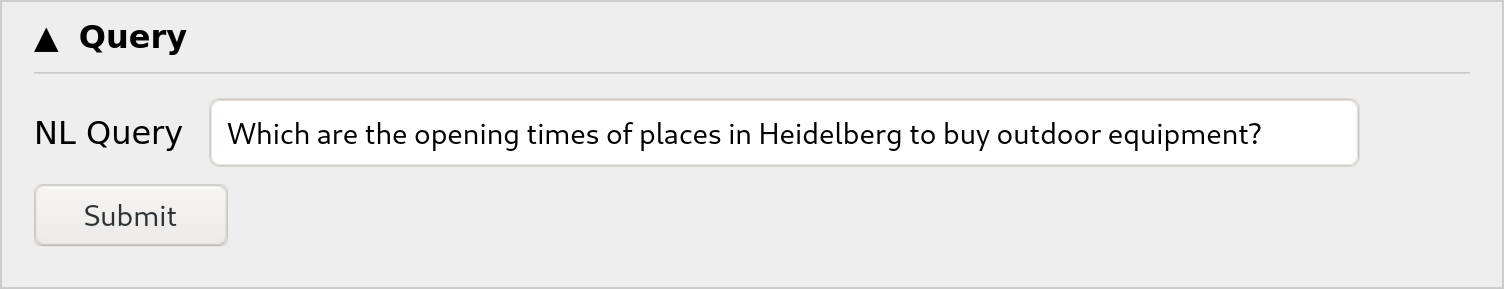
\includegraphics[width=0.7\textwidth]{fig/screenshot_outdoor_nl.png}
    \caption{User enters NL query.}
  \end{subfigure}
  \begin{subfigure}{\textwidth}
    \centering
    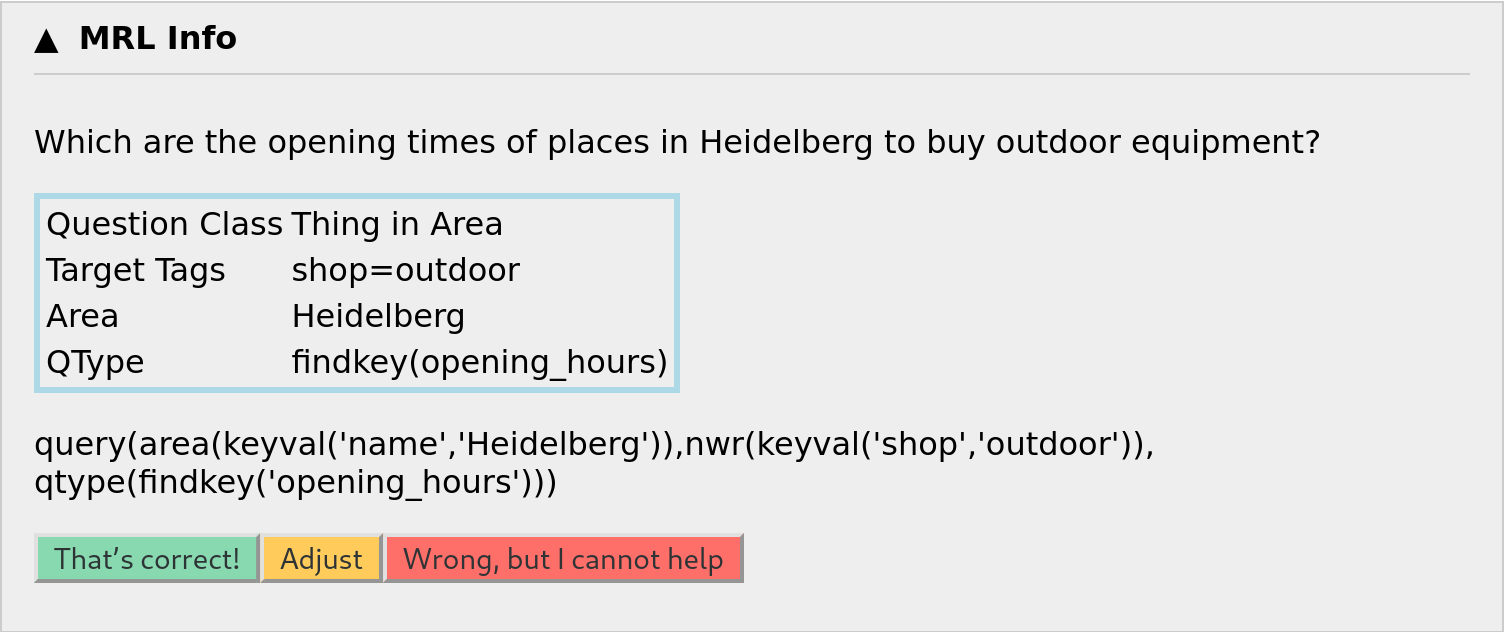
\includegraphics[width=0.7\textwidth]{fig/screenshot_outdoor_mrl.png}
    \caption{Info about MRL query the parser produced.}
  \end{subfigure}
  \begin{subfigure}{\textwidth}
    \centering
    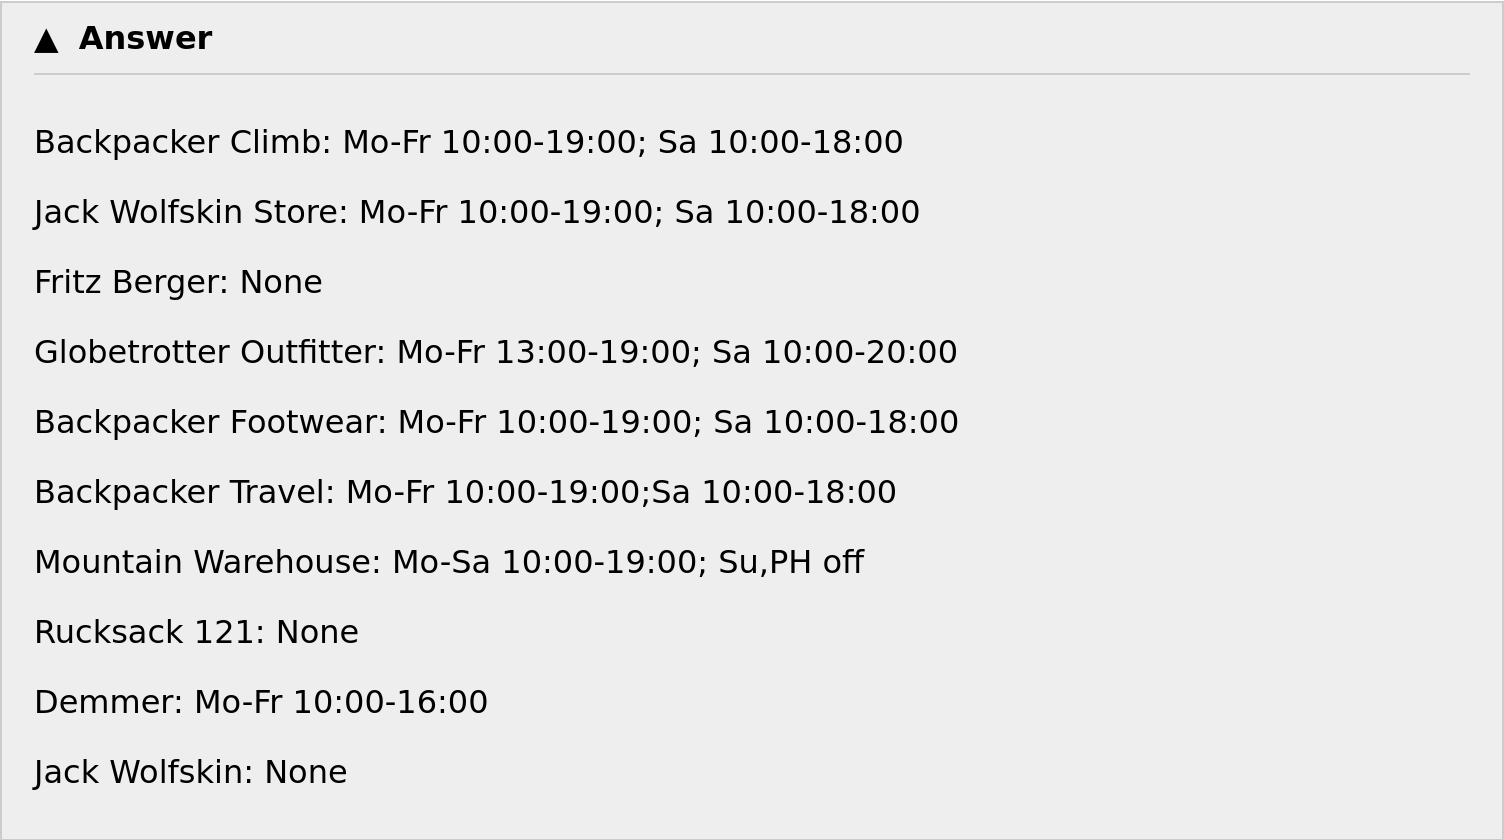
\includegraphics[width=0.7\textwidth]{fig/screenshot_outdoor_answer.png}
    \caption{Answer of the query.}
  \end{subfigure}
  \begin{subfigure}{\textwidth}
    \centering
    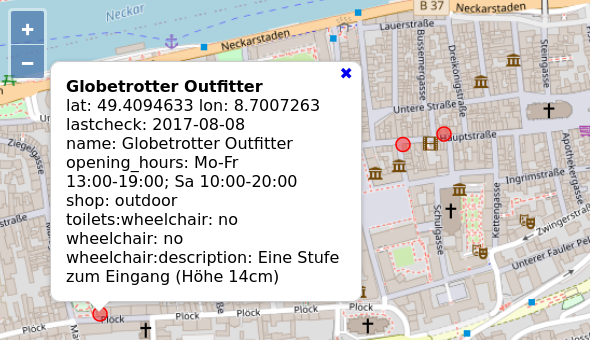
\includegraphics[width=0.7\textwidth]{fig/screenshot_outdoor_map.png}
    \caption{Interactive map of the results.}
  \end{subfigure}
  \caption[Successful query process]{Successful query process with the NL query
    \nl{Which are the opening times of places in Heidelberg to buy outdoor
      equipment?}.}
  \label{fig:successful-query-process}
\end{figure}

\begin{figure}[h]
  \centering
  \begin{subfigure}{\textwidth}
    \centering
    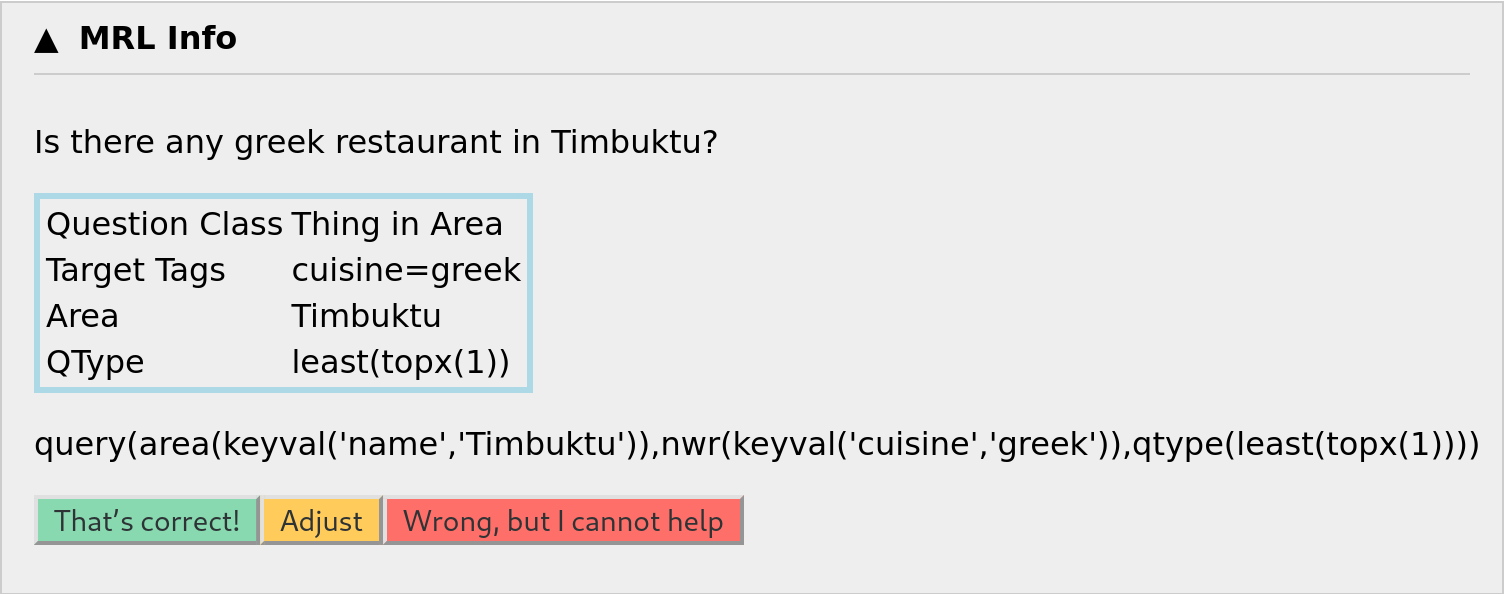
\includegraphics[width=0.7\textwidth]{fig/screenshot_greek_mrl.png}
    \caption{MRL Info missing the \osmtag{amenity=restaurant} tag.}
  \end{subfigure}
  \begin{subfigure}{\textwidth}
    \centering
    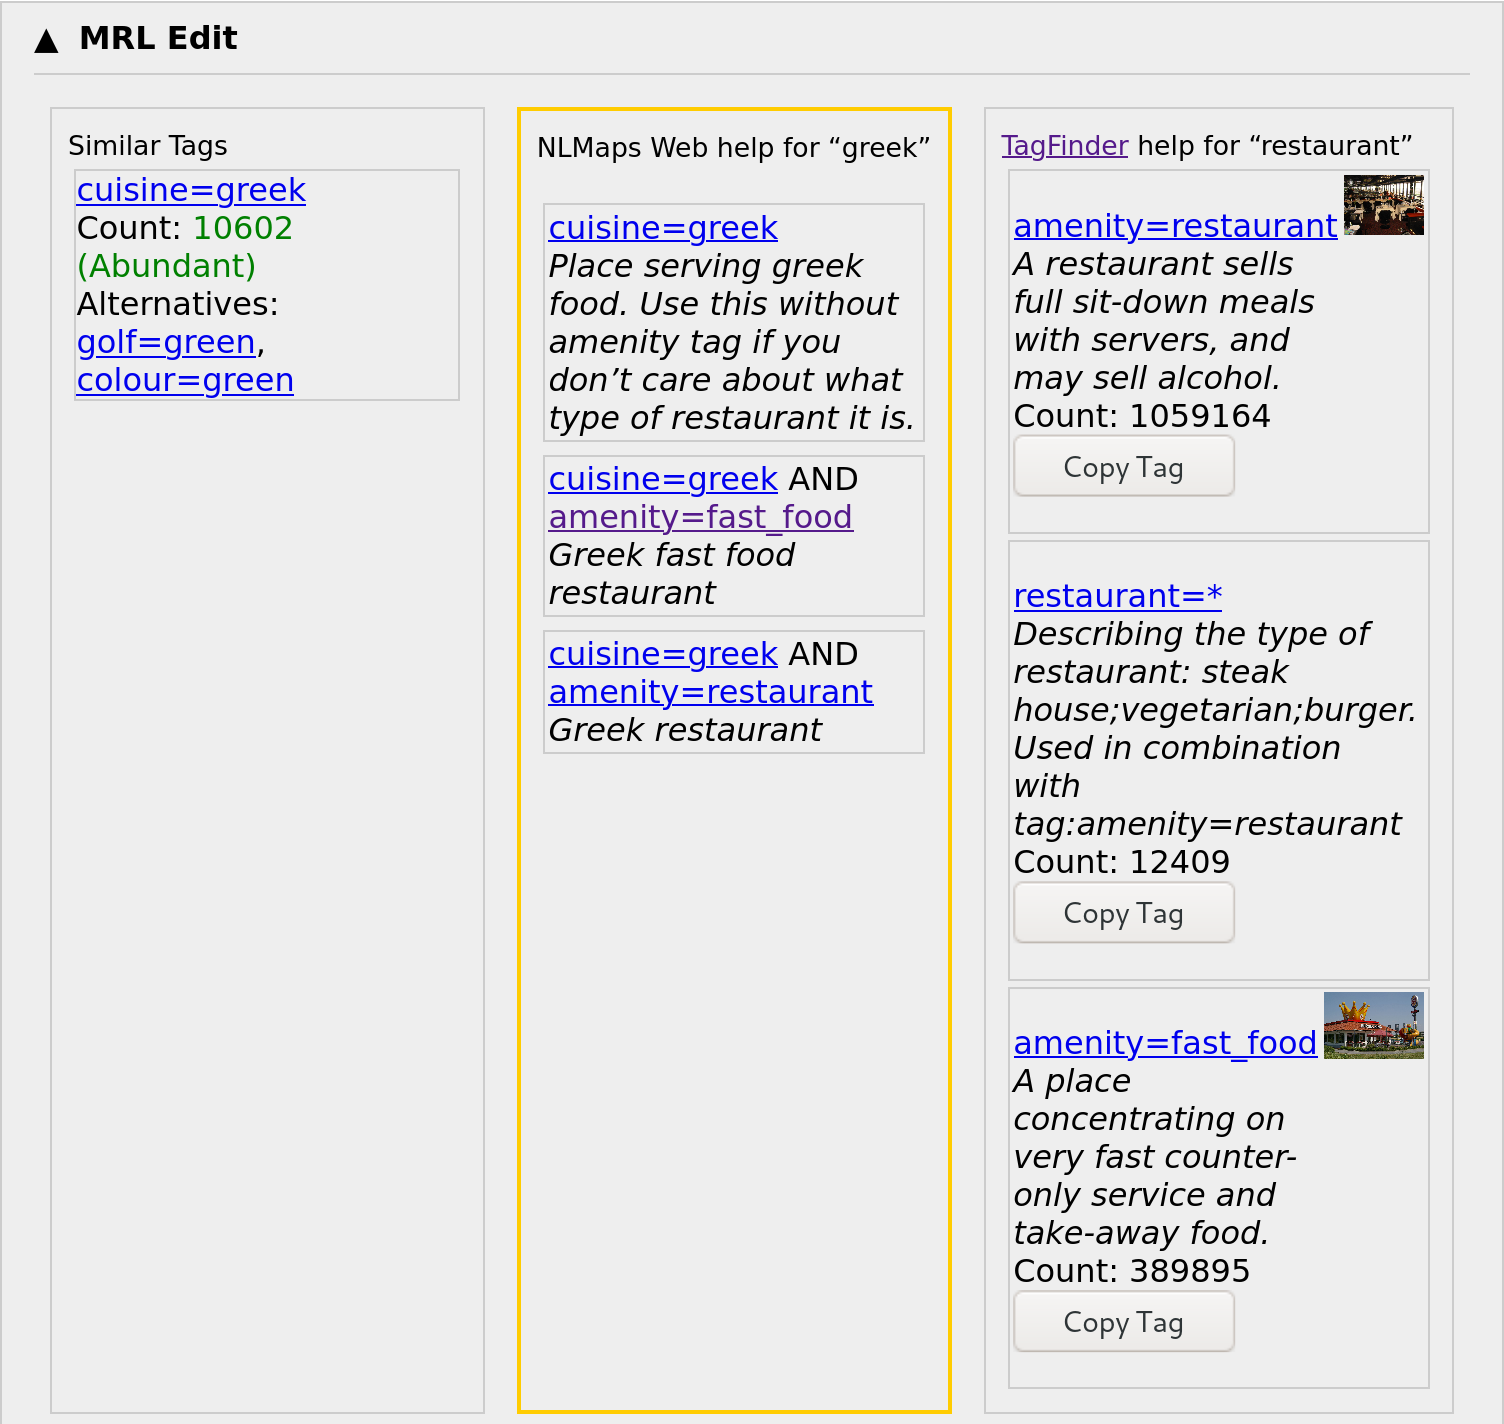
\includegraphics[width=0.7\textwidth]{fig/screenshot_greek_help.png}
    \caption{Help for the user showing tags with similar spelling, custom
      suggestions for the keyword \emph{greek} and TagFinder suggestions for
      \emph{restaurant}.}
  \end{subfigure}
  \begin{subfigure}{\textwidth}
    \centering
    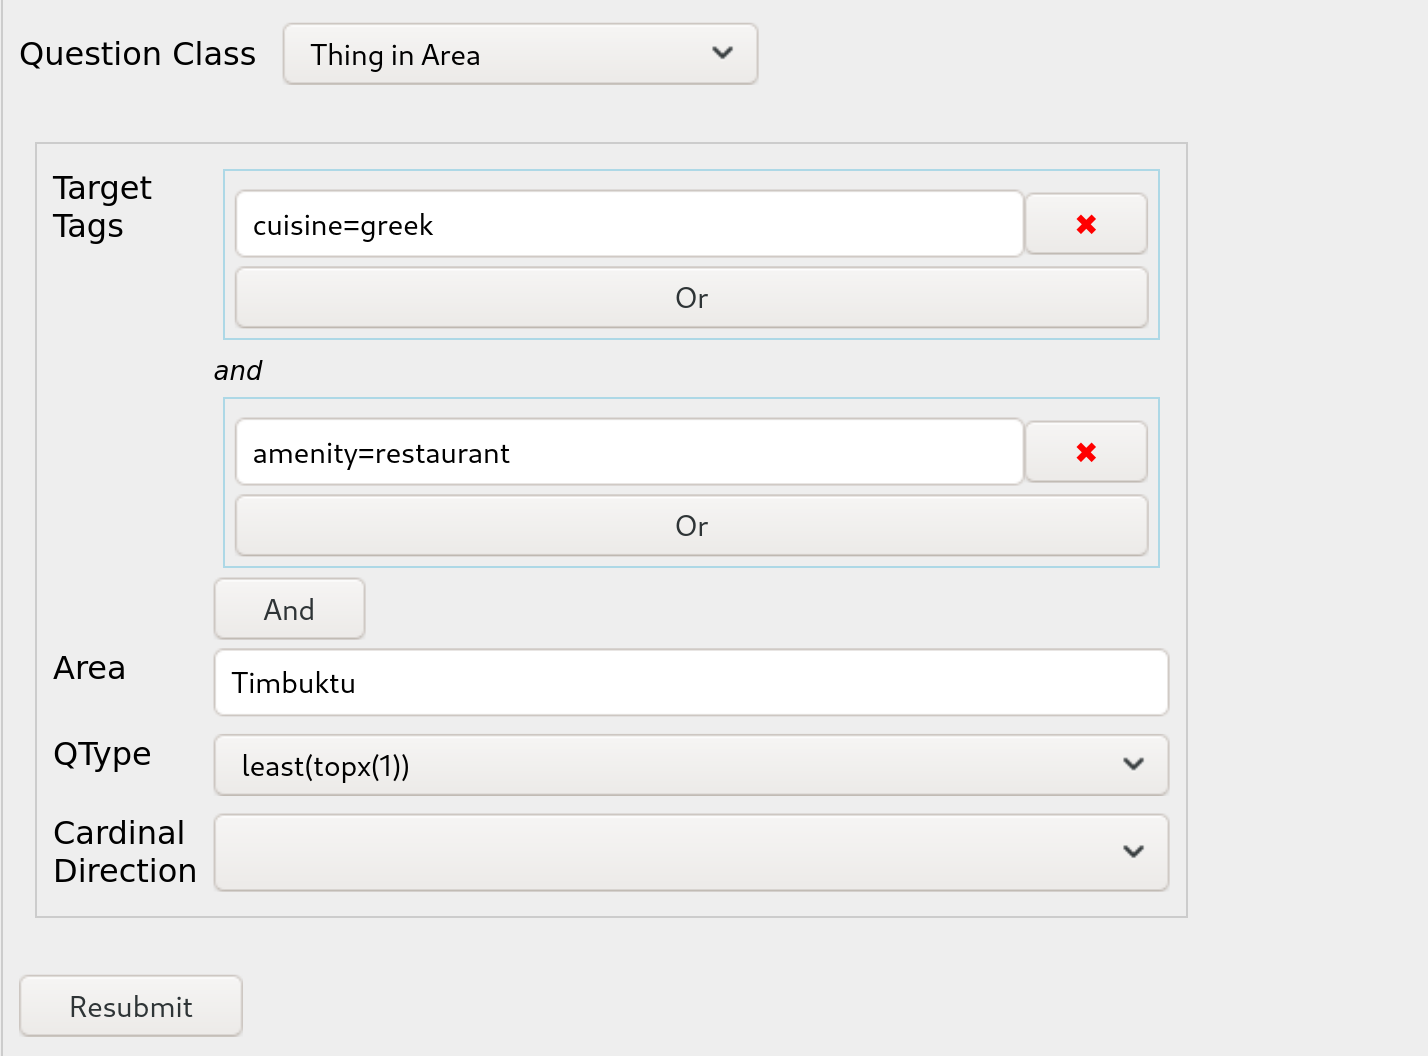
\includegraphics[width=0.7\textwidth]{fig/screenshot_greek_form.png}
    \caption{Form where the user added \osmtag{amenity=restaurant}.}
  \end{subfigure}
  \caption[MRL correction process]{MRL correction process after asking \nl{Is
      there any greek restaurant in Timbuktu?}.}
  \label{fig:correction-process}
\end{figure}

\section{Architecture}

Instead of being one large system, \nlmapsweb{} is split into two parts: First,
the web interface the user interacts with, which also handles user management,
giving tag help, displaying answers, logging queries and a tutorial. Second, the
parsing server that parses NL queries into MRL queries, trains and updates the
model based on feedback received through the web interface and also stores that
feedback. They are separated so that the machine that runs the web server is not
required to also handle running or even training a neural network, which is a
resource-intensive task that is usually parallelized on a GPU. Because of the
separation, it is possible to use a small machine for the web interface that
interacts with the parsing server running on a GPU cluster, which may only be
accessible by SSH and thus be unreachable through a
well-known\footnote{\url{https://en.wikipedia.org/wiki/List_of_TCP_and_UDP_port_numbers\#Well-known_ports}.}
HTTP port.

Both systems are implemented as HTTP Servers with the Python web framework
Flask\footcite{flask} and employ SQLite\footcite{sqlite} as their database. The
parsing server exposes a JSON-based HTTP API, which is used by the web
interface. The parsing server wraps the PyTorch\footcite{pytorch}-based
sequence-to-sequence learning framework Joey NMT\footcite{joeynmt}
\parencite{kreutzer-2019}.

Figure~\ref{fig:querying-architecture} shows the basic querying flow through the
architecture: The user enters their NL query into the web interface, which calls
on the parsing server to parse it into an MRL. The MRL is used to retrieve the
answer via the MRL interpretation package (cf.
Section~\ref{sec:mrl-interpretation}) and the web interface sends the MRL query
along with the retrieved answer in its response to the user.

\begin{figure}[h]
  \centering
  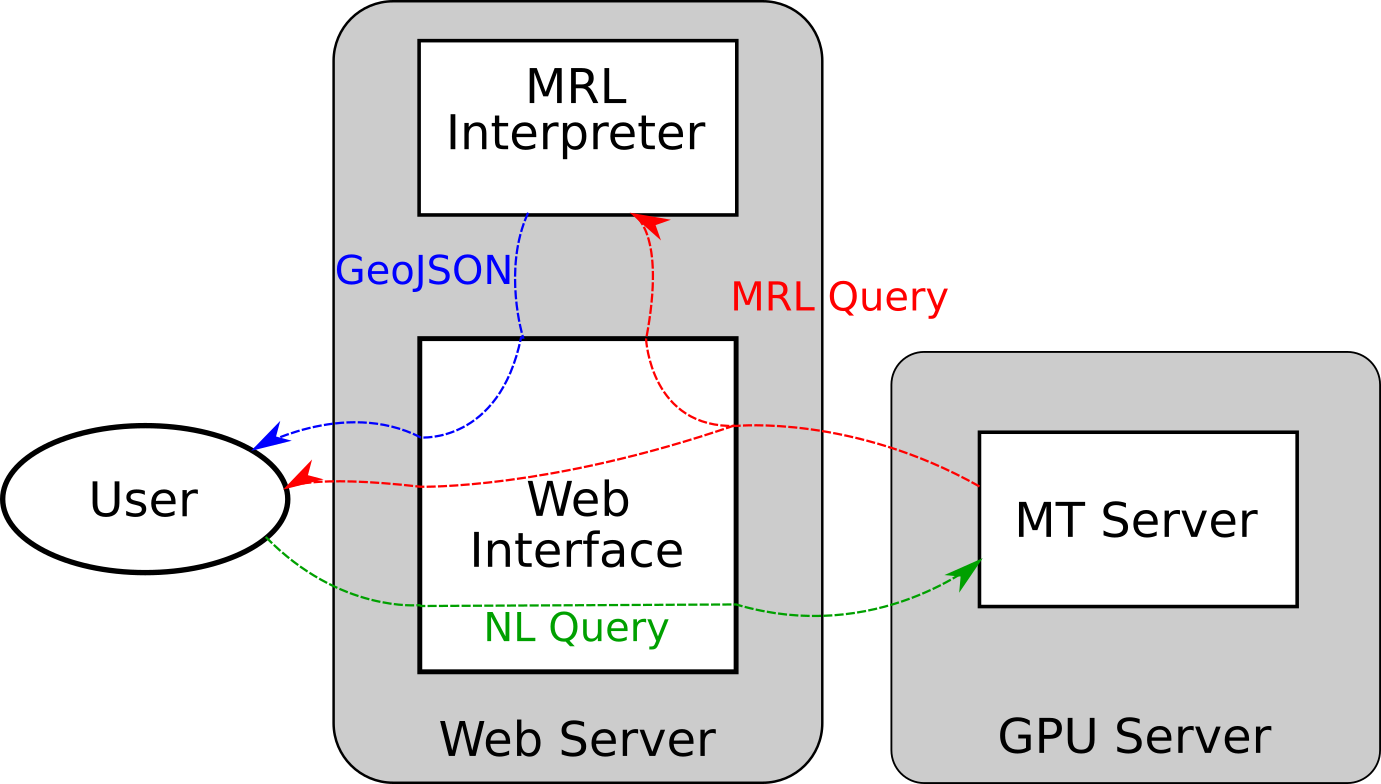
\includegraphics[width=\textwidth]{fig/querying_architecture.png}
  \caption[Querying Architecture]{System Architecture for Querying}
  \label{fig:querying-architecture}
\end{figure}

As shown in Figure~\ref{fig:learning-architecture}, the web interface also
extracts the keywords from the NL query (cf.
Section~\ref{sec:keyword-extraction}) and suggests tags based on them. With this
information, the user can correct the MRL if it is wrong and can send their
feedback in the form of a correct NL-MRL query pair to the web interface. The
feedback is then sent to the parsing server in order to initiate the training
procedure and to update the model.

\begin{figure}[h]
  \centering
  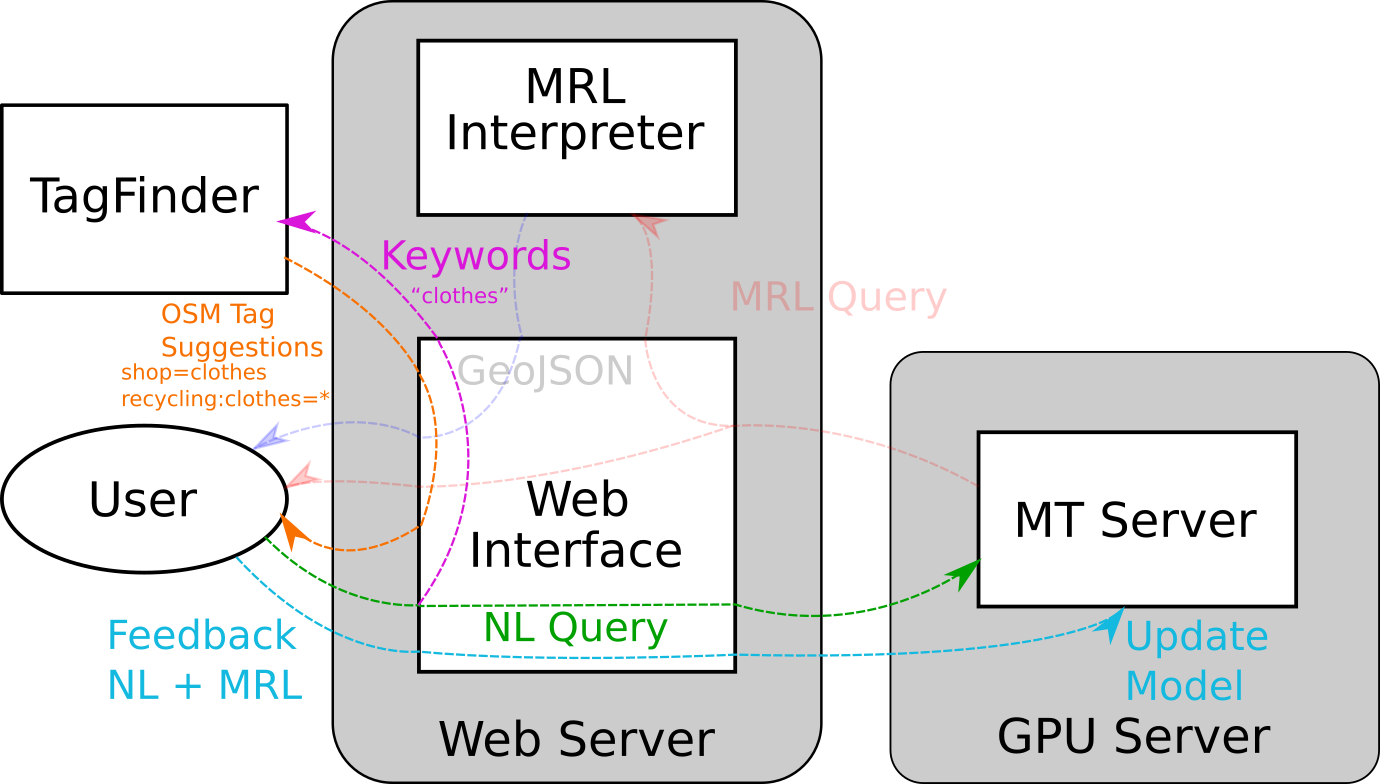
\includegraphics[width=\textwidth]{fig/learning_architecture.png}
  \caption[Feedback \& Learning Architecture]{System Architecture for Feedback
    and Learning}
  \label{fig:learning-architecture}
\end{figure}

\section{MRL Interpretation}
\label{sec:mrl-interpretation}

In the course of their foundational work, \textcite{haas-2016}
forked\footcite{online-overpass-nlmaps} the Overpass API and included
functionality for reading an MRL query and executing the Overpass QL queries
necessary to answer it. Unfortunately, there are three problems with this
approach.

\begin{itemize}
\item Their fork has been unmaintained for years and thus does not profit from
  further development and bugfixes in the upstream Overpass API project. Merging
  the upstream bugfixes and other changes and maintaining the fork would mean a
  lot of ongoing work.
\item Running an instance of the Overpass API entails having a complete copy of
  OSM data stored in the Overpass database and keeping it up to date, which also
  is a lot of work.
\item The Overpass API is meant for precise queries to the OSM database and has
  no functionality for fuzzy matching of place names\footnote{Regular
    expressions are supported, but they do not suffice for this task.} or for
  ranking results by importance. These are typical cases where this becomes a
  problem:
  \begin{itemize}
  \item The user asks \nl{Show Verpackungsmuseum in Heidelberg} and the parser
    correctly analyzes that the user wants a place called
    \emph{Verpackungsmuseum}. However, the Overpass API will not find such a
    place because that museum is in fact called \emph{Deutsches
      Verpackungsmuseum}.
  \item The user asks for objects in \emph{Paris}, but there are several cities
    with that name in the world and the Overpass API has no importance ranking
    with which it could determine that the capital of France is most likely the
    city the user has in mind.
  \end{itemize}
\end{itemize}

Instead of using the forked version for answering MRLs, a Python module is
developed for that task. In a first step, the area requested in the query is
looked up in Nominatim, which supports fuzzier search than the Overpass API and
also ranks the results by an importance score. Second, the named reference
location is looked up if there is one in the query (e.g. \emph{Eiffel Tower} in
\nl{bars near Eiffel Tower in Paris}). This is also done via Nominatim and the
results are restricted to the area that was selected in the previous step.
Finally, an Overpass QL query is generated where the previously retrieved area
and reference location are selected by their OSM ID instead of their name. This
query is then sent to any of the publicly available Overpass API instances for
retrieving the result, which means that there is no need of running a separate
instance of the API with all the maintenance work.

% TODO: Link to Repo
% TODO: Example.

\section{NL Query Keyword Extraction}
\label{sec:keyword-extraction}

In order to suggest tags for the user to use when correcting a faulty MRL query,
the most relevant keywords are extracted from their NL query so that the
keywords can be looked up in the TagFinder. Assuming that a relevant keyword is
a term occurring in that query that does not occur in a lot of other queries, we
turn to \(\tfidf\) for ranking the terms.

For a term \(t\) in an NL query \(d\), its \(\tfidf\) score is calculated as
\begin{align}
  \tfidf (t, d, D) = \tf(t, d) \times \idf(t, D)
\end{align}
where the collection of all NL queries in \nlmapsthree{} is used as the
reference document set \(D\). The term frequency \(\tf(t, d)\) is the raw count
of term \(t\) in the NL query \(d\) and the inverse document frequency is
calculated as
\begin{align}
  \idf(t, D) = \ln \frac{N + 1}{\df(t, D) + 1} + 1
\end{align}
where \(N = \cardinality{D}\) is the number of NL queries in \(D\) and \(df(t, D) =
\cardinality{\left\{ d \in D : t \in d \right\}}\) is the number of NL queries
containing the term \(t\). \num{1} is added in the numerator and in the
denominator for smoothing over unseen terms and a further \num{1} is added in
order not to completely disregard terms that occur in every NL query.

Any terms with a score \(\tfidf(t, d, D) > 0.3\) (the cutoff was determined
manually) are looked up in TagFinder except if they occur in a separate list of
stop words or if they are part of a location name, which is determined by using
the MRL query returned by the parser.

% TODO: Example

\section{Online Learning}

%%% Local Variables:
%%% coding: utf-8
%%% mode: latex
%%% TeX-engine: xetex
%%% TeX-parse-self: t
%%% TeX-command-extra-options: "-shell-escape"
%%% TeX-master: "../thesis"
%%% End: